\section{Poisson's Equation and Laplace's Equation}
\subsection{The boundary value problem}
Many equations in mathematical physics can be
reduced to one of the form
\begin{definition}[Poisson's equation, Laplace's equation]
    The \textbf{Poisson's equation} is
    \[
      \nabla^2 \varphi = F,
    \]
    where $F$ is given and $\varphi$ is to be solved. When $ F=0 $, the equation becomes 
    \[
        \laplacian \varphi = 0,
    \]
    which is called the \textbf{Laplace's equation}.
\end{definition}

This equation either needs to be solved on all of $ \mathbb{R}^{n} $, or some domain $ \Omega \subseteq \mathbb{R}^{n} $, where $n=2,3$.

Physical problems involve boundary conditions, so to solve Poisson's equation we need to prescribe some boundary conditions for the function $\varphi$ on the boundary $\partial \Omega,$ or as $|\mathbf{x}| \rightarrow \infty$ if solving on all of $\mathbb{R}^{n}$. 

The \textbf{Dirichlet problem} for Poisson's equation is
\[
    \begin{cases}
        \nabla^{2} \varphi =F&\text {in } \Omega \\
        \varphi =f&\text {on } \partial \Omega\\
    \end{cases} 
\]
and the \textbf{Neumann problem} is
\[
    \begin{cases}
        \nabla^{2} \varphi =F  &\text {in } \Omega \\
        \dfrac{\partial \varphi}{\partial \mathbf{n}}=g & \text {on } \partial \Omega\\
    \end{cases} 
\]
Here we have used the normal derivative
\[
    \frac{\partial \varphi}{\partial \mathbf{n}} \equiv \mathbf{n} \cdot \nabla \varphi.
\]

It is important to interpret the boundary conditions in an appropriate way: we assume that $ \varphi $ \textit{continuously} approaches the boundary data as $\mathbf{x}\to\partial \Omega$, i.e. we assume that \textit{$\varphi$ and $\nabla \varphi$ are continuous on the set $\Omega \cup \partial \Omega$}.

\begin{remark}
    If $ \laplacian \varphi=0 $ in $ \Omega $, then $ \varphi $ needs to be well-defined on all of $ \Omega $. Don't fall into trap of assuming things like
    \[
        \laplacian\left( \frac{1}{|\bfx|} \right)=0,\quad \forall \bfx\in \mathbb{R}^{3}.
    \]
    It is only true for $\bfx\neq \mathbf{0}$ (check this). So when we’re talking about solutions to Laplace’s equation, we’re necessarily talking about functions which are non-singular. 
\end{remark}

\begin{example}
    Let $ r=|\bfx| $. Consider boundary value problem 
    \[\tag{$*$}
        \begin{cases}
        \laplacian \varphi=r &\text{in }r<a\\
        \varphi=1 &\text{on }r=a\\
        \end{cases} 
    \]
    The spherical symmetry suggests we look for a solution of the form $ \varphi=\varphi(r) $. Substituting in and using the fact for pherically symmetric $ \varphi $ we have 
    \[
        \nabla^{2} \varphi=\frac{1}{r^{2}} \frac{\mathrm{d}}{\mathrm{d} r}\left(r^{2} \frac{\mathrm{d} \varphi}{\mathrm{d} r}\right),
    \]
    we see that our problem is equivalent to
    \[
        \left(r^{2} \varphi^{\prime}\right)^{\prime}=r^{3}, \quad \varphi(a)=1.
    \]
    General solution to $(*)(\rma)$ is 
    \[
        \varphi(r)=A+\frac{B}{r}+\frac{1}{12}r^3.
    \]
    We must have $B=0$ since $ \varphi $ is defined on all of $ \{r<a\} $. So using $ (*)(\rmb) $ we get $ A=1-\frac{a^3}{12} $, and the solution is 
    \[
        \varphi(r) = 1+\frac{1}{12}(r^3-a^3).
    \]
\end{example}

\begin{note}
    In general, we want problems in mathematical physics to be \textit{well-posed} (by Hadamard): 
    \begin{enumerate}
        \item Want solutions to \textit{exist}.
        \item Want solutions to be \textit{unique}.
        \item Want solutions to have \textit{continuous} dependence on initial or boundary conditions.
    \end{enumerate}
    The reasons to 1 and 2 are easy to interpret. For 3, note that in real life we use apparatus to measure things and justify theories.
    \begin{center}
        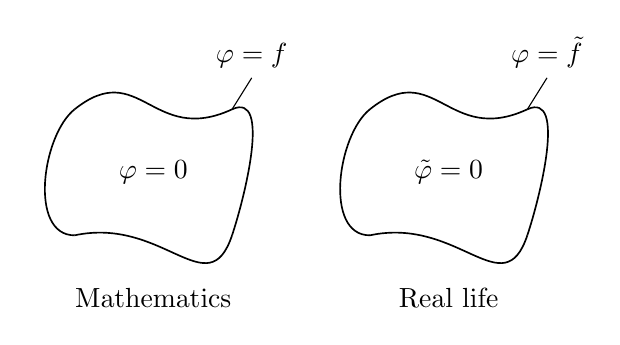
\begin{tikzpicture}[yscale=0.8]
            \node (0) at (-1, 1) {};
            \node (1) at (1, 1) {};
            \node (2) at (1, -1) {};
            \node (3) at (-1, -1) {};
            \node (4) at (0, 0) {$\laplacian \varphi=0$};
            \node (5) at (1.25, 1.5) {};
            \node [above] at (5) {$\varphi=f$};
            \node (6) at (0, -2) {Mathematics};
            \node (7) at (2.75, 1) {};
            \node (8) at (4.75, 1) {};
            \node (9) at (4.75, -1) {};
            \node (10) at (2.75, -1) {};
            \node (11) at (3.75, 0) {$\laplacian \tilde{\varphi}=0$};
            \node (12) at (5, 1.5) {};
            \node [above] at (12) {$\varphi=\tilde{f}$};
            \node (13) at (3.75, -2) {Real life};
            \draw [semithick, in=-150, out=45, looseness=1.50] (0.center) to (1.center);
            \draw [semithick, in=75, out=30, looseness=0.75] (1.center) to (2.center);
            \draw [semithick, in=15, out=-105, looseness=1.50] (2.center) to (3.center);
            \draw [semithick, in=-135, out=-180, looseness=0.75] (3.center) to (0.center);
            \draw (5.center) to (1.center);
            \draw [semithick, in=-150, out=45, looseness=1.50] (7.center) to (8.center); 
            \draw [semithick, in=75, out=30, looseness=0.75] (8.center) to (9.center);
            \draw [semithick, in=15, out=-105, looseness=1.50] (9.center) to (10.center);
            \draw [semithick, in=-135, out=-180, looseness=0.75] (10.center) to (7.center);
            \draw (12.center) to (8.center);
        \end{tikzpicture}
    \end{center}
    The error would be $ \| f-\tilde{f} \| $, which we want to be \textit{small}. i.e. we want $ \|\varphi-\tilde{\varphi}\| $. In this course we mainly care about 2.
\end{note}

We only want to solve problems that have a unique, or almost unique solution. Let us consider a generic \textit{linear} problem of the form
\[
    \begin{cases}
        L \varphi=F & \text {in } \Omega \\
        B \varphi=f & \text {on } \partial \Omega
    \end{cases} 
\]
for some \textit{linear} differential operators $L$ and $B$. If $\varphi_{1}$ and $\varphi_{2}$ are two different solutions to this problem, then their difference, $\psi=\varphi_{2}-\varphi_{1}$, must satisfy the homogeneous problem
\[
    \begin{cases}
        L \psi=0 & \text {in } \Omega \\
        B \psi=0 & \text {on } \partial \Omega
    \end{cases} 
\]
If we can show that the only solution to this problem is $\psi=0$, we will have to conclude that $\varphi_{1}=\varphi_{2},$ i.e. the solution to the original problem is unique. The moral of the story is 
\begin{quote}
    \textit{The solution to a linear problem is unique iff the only
    solution to homogeneous problem is the zero solution.}
\end{quote}

\begin{proposition}
    The solution to the Dirichlet problem is unique. The solution to the Neumann problem is unique upto addition of a constant.
\end{proposition}
\begin{proof}
    Let $ \psi=\varphi_1-\varphi_2 $ be the difference of 2 solutions to Dirichlet or Neumann problems, so 
    \[
    \begin{cases}
        \laplacian \psi=0 & \text {in } \Omega \\
        B \psi=0 & \text {on } \partial \Omega
    \end{cases} 
    \]
    where $B \psi \equiv \psi$ (Dirichlet) or $B \psi \equiv \frac{\partial \psi}{\partial n}$ (Neumann). Consider the non-negative functional
    \[
        I[\psi]=\int_{\Omega}|\nabla \psi|^{2} \mathrm{~d} V \ge 0
    \]
    Clearly $I[\psi]=0$ if and only if $\nabla \psi=0$ on $\Omega$. Note that
    \[
        I[\psi]=\int_{\Omega} \nabla \psi \cdot \nabla \psi \mathrm{~d} V=\int_{\Omega}\left(\nabla \cdot(\psi \nabla \psi)-\psi \nabla^{2} \psi\right) \mathrm{d} V.
    \]
    The second term vanishes because $\nabla^{2} \psi=0$ in $\Omega$. Using the divergence theorem on the first term, we find
    \[
        I[\psi]=\int_{\partial \Omega} \psi \frac{\partial \psi}{\partial \mathbf{n}} \mathrm{~d} S=0.
    \]
    Hence $\nabla \psi=0$ throughout $\Omega,$ i.e. $\psi$ is constant. We then have two cases to consider:
    \begin{enumerate}[(a)]
        \item In the Dirichlet case, $\psi=0$ on the boundary. By continuity of $\psi$ on $\Omega \cup \partial \Omega$ we conclude $\psi=0$ throughout $\Omega$. So the solution to the Dirichlet problem is unique.
        \item In the Neumann case we only know that $\frac{\partial \psi}{\partial \bfn}=0$ on $\partial \Omega,$ so we cannot say any more than $\psi=\text{const}$ throughout $\Omega$. So the solution to the Neumann problem is unique upto the addition of a constant.\qedhere
    \end{enumerate}
\end{proof}

\begin{example}
    From electrostatics, consider charge density
    \[
        \rho(\bfx) = \begin{cases}
        0 &r<a\\
        F(r) &r\ge a\\
        \end{cases} 
    \]
    \begin{claim}
        There is no electric field in $ r<a $.
    \end{claim}
    Indeed, we know that the electric potential $ \phi $ satisfies 
    \[
        \laplacian \phi = -\frac{\rho(\bfx)}{\epsilon_0}=0,\quad r<a.
    \]
    By spherical symmetry, $ \phi=\phi(r) $, so $ \phi=\phi(a)=\phi_0=\text{const} $ on $ r=a $. Note that one solution to 
    \[
        \begin{cases}
        \laplacian \phi=0 &r<a\\
        \phi=\phi_0 &r=a\\
        \end{cases} 
    \]
    is $ \phi=\phi_0 $. Since $\phi$ is constant throughout $r < a$, $\bfE(\bfx) = - \nabla \phi= \mathbf{0}$.
\end{example}

The same example holds if we replace electrostatics with gravity. We’ve essentially just proved \textbf{Newton’s shell theorem}: there is no net gravitational field anywhere inside a spherical shell. Newton’s proof was significantly more involved, but only used elementary concepts from geometry. It’s also not very rigorous.